\begin{frame}
	\frametitle{Proposta}
	\par Construir uma visualização que, além dos gráficos de linha e energia, remeta ao posicionamento dos eletrodos no sistema 10-20 \textbf{sem} o uso de gradientes e que permita:
	\begin{columns}
		\begin{column}{0.42\textwidth}
			\begin{itemize}
				\item selecionar o sujeito e estímulo (interatividade)
				\item visualizar de forma geral e particular cada um dos sinais captados pelos sensores (interatividade)
				\item exibir a origem do sinal
				\item ampliar as curvas geradas (visualizar detalhes)
				\item mostrar o energia total do sinal no intervalo mostrado
				\item uso de cores com alto contraste (percepção)
			\end{itemize}
		\end{column}
		\begin{column}{0.66\textwidth}
			\only<1>{
				\begin{figure}
					\centering
					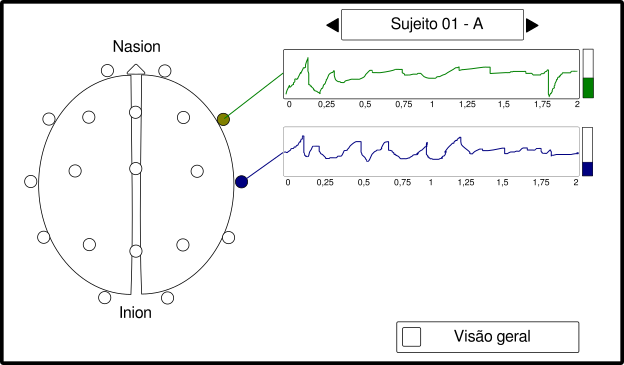
\includegraphics[width=\linewidth]{images/g3714}
					\caption{Visão geral}
					\label{fig:g3714}
				\end{figure}
			}
			\only<2>{
				\begin{figure}
					\centering
					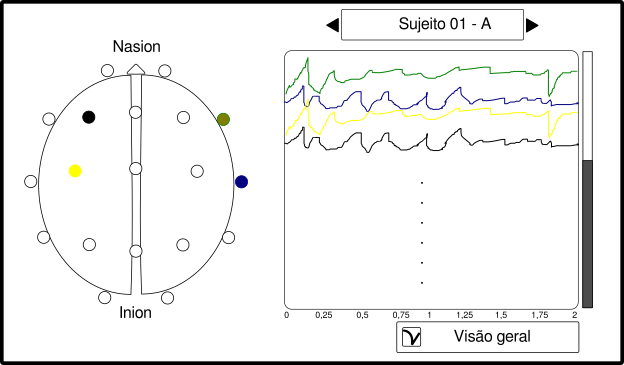
\includegraphics[width=\linewidth]{images/g3762}
					\caption{Visão específica}
					\label{fig:g3762}
				\end{figure}
			}
		\end{column}
	\end{columns}
\end{frame}
\begin{frame}[allowframebreaks]
	\frametitle{Discussão da proposta}
	\par Tanto a \textbf{seleção do sujeito e estímulo} quanto o a caixa e checagem fazem parte do \textbf{ciclo de visualização} (loop), dessa forma, ao mudar o tipo de visão e/ou o sujeito analisado se tem uma resposta imediata na visualização.\newline
	
	\par As cores de \textbf{alto contraste} permitem localizar a origem dos dados facilmente evitando um problema comum que é a diferenciação dos dados quando cores muito similares são usadas.\newline
	
	\par A \textbf{ampliação} permite que cada sinal possa ser visto em \textbf{detalhes}, dessa forma, fica mais fácil visualizar as informações vinculadas aos sinais de baixa e alta frequência proporcionando a identificação de \textbf{objetos segundo sua "silhueta"}.\newline
	
	\par Vale destacar que os atributos usados na proposta tem uma ordenção \textbf{sequêncial} para a amplitude e frequência dos sinais durante o tempo (gráficos de linha) e ao mesmo tempo é \textbf{categórico} pois a análise das frequências podem dizer muito sobre o sujeito que está sendo analizado.\newline
	\par O atributo de energia (barra vertical lateral ao gráfico de linhas) é \textbf{quantitativo}.\newline
	
	\par Em se tratando de atributos \textbf{categóricos} vale destacar também a região à direita dos gráficos. Essa seção indica quais regiões do cérebro estão enviando quais sinais, dessa forma, é possível, por exemplo, inferir quais regiões do cérebro estão mais ativas quando da execução de algum pensamento e/ou ação.\newline
	
	\par Nota-se a \textbf{proximidade} utilizada da barras laterais com seus respectivos gráficos de linha.\newline
	
	\par Em termos de \textbf{categorias semióticas} \cite{santaella2017semiotica} é possivel destacar:
	\begin{itemize}
		\item primeiridade: Cores que destacam e chamam imediatamente a atenção do usuário ou usuária.
		\item secundidade: O conjunto ação/reação aplicado aos controles e imagens.
		\item terceiridade: A consequente interpretação da imagem apresentada assim como os raciocínios necessários para o entendimento do que é mostrado.
	\end{itemize}

\end{frame}